\documentclass[11pt,oneside]{book}

\usepackage{amsthm, amsmath, amssymb, mathrsfs, graphicx, tabularx, multirow, algorithm, algorithmicx, algpseudocode}
\usepackage[pdfborderstyle={/S/S}]{hyperref}
\usepackage{hyperref}

\DeclareMathOperator*{\argmax}{arg\,max}
\DeclareMathOperator*{\argmin}{arg\,min}
\DeclareMathOperator{\permindex}{index}
\DeclareMathOperator{\Inv}{Inv}
\DeclareMathOperator{\probability}{P}
\DeclareMathOperator{\expectedvalue}{E}
\DeclareMathOperator{\meet}{\wedge}
\DeclareMathOperator{\bigmeet}{\bigwedge}
\DeclareMathOperator{\join}{\vee}
\DeclareMathOperator{\bigjoin}{\bigvee}
\DeclareMathOperator{\symmetricdifference}{\vartriangle}

\theoremstyle{plain}
\newtheorem{theorem}{Theorem}
\newtheorem{lemma}[theorem]{Lemma}
\newtheorem{proposition}[theorem]{Proposition}
\newtheorem{corollary}[theorem]{Corollary}
\newtheorem{openproblem}{Open Problem}

\theoremstyle{definition}
\newtheorem{definition}{Definition}[section]
\newtheorem{conjecture}{Conjecture}[section]
\newtheorem{example}{Example}[section]

\theoremstyle{remark}
\newtheorem*{remark}{Remark}
\newtheorem*{note}{Note}
\newtheorem{case}{Case}
\newtheorem{claim}{Claim}

\let\emptysetraw\emptyset
\renewcommand{\emptyset}{\varnothing}

\begin{document}

\frontmatter

\title{A Generalized Probabilistic Gibbard-Satterthwaite Theorem}
\author{Jonathan Potter \\ jmp2909@rit.edu}
\date{
	\today \\
	\vspace{3in} \small
	\begin{center}
		\begin{tabular}{rl}
			\emph{Chair} & Christopher Homan \\
			\emph{Reader} & Ivona Bez\'{a}kov\'{a} \\
			\emph{Observer} & Zack Butler
		\end{tabular}
	\end{center}
}

\maketitle

%!TEX root = thesis.tex

\chapter*{Abstract}

Friedgut, Kalai, and Nisan have proved that social choice functions can be successfully manipulated by random preference reordering with non-negligible probability \cite{friedgut2008elections}. However, their results require two restrictions: the social choice function must be neutral, and the election must have at most 3 alternatives. In this thesis we focus on removing the latter restriction and generalizing the results to elections with any number of candidates. We also provide a survey of related work analyzing and comparing results from a number of authors.

%!TEX root = thesis.tex

\chapter*{Acknowledgments}

First and foremost, I would like to thank my advisor, Christopher Homan, without whom this work and my academic endeavors would have been greatly diminished. Thank you for many, many hours of instruction, encouragement, and challenging me to better myself. You have made this an enjoyable experience and I have learned and grown in leaps and bounds, both academically and otherwise.

Second, I would like to thank my family---which I am so lucky to be a part of---whose love and support undergird all of my endeavors.


\hypersetup{
	pdfborderstyle={}
}

\tableofcontents
% \listoffigures
% \listoftables

\hypersetup{
	pdfborderstyle={/S/S}
}

\mainmatter

%!TEX root = thesis.tex


\chapter{Introduction}

	In this thesis we endeavor to extend the results of Friedgut, Kalai, and Nisan \cite{friedgut2008elections} who proved that social choice functions can be successfully manipulated by random preference reordering with non-negligible probability. However, there are two main restrictions on their results: the social choice function must be neutral, and the election must have at most 3 alternatives. We attempt to remove the later restriction in order to generalize the results to elections with any number of candidates.

	Our proof draws upon many aspects of Friedgut, Kalai, and Nisan's proof. Their proof is done in three steps, with the first two steps being already written in general terms, while the third is restricted to 3 alternatives. Therefore we need only generalize the third step. We rely heavily on lattice theory and combinatorics to prove this generalization.


\section{Importance}

	It is obvious, and widely accepted that election systems are important to society. They are essential to democracy which is the foundation of many nations' governments, and are also used in many non-political situations---anywhere a group of independent agents needs to come to a consensus. They are used in schools, electing board members for a business, and stock holders voting on issues affecting a company. Election systems are not even wholly reserved to humans. Elections can be used by artificial intelligence systems when a group of agents needs to make a decision \cite{ephrati1991clarke, ephrati1993multi, pennock2000social, dwork2001rank, fagin2003efficient}, and they can be used in internet page ranking algorithms for search engines \cite{chevaleyre2007short}.

	However, it is less clear that manipulation in elections---especially random manipulation---is important, so we will attempt to describe its importance by briefly explaining the history behind it.

	One obvious criteria for a good election system is fairness \cite{chevaleyre2006issues}, and it is generally accepted that the winning candidate should, on the whole, represent the will the constituents'. It is easy to recognize a fair election system if there are only two candidates: the candidate who is preferred by the majority of voters should win. But with a larger number of candidates, determining the fairness of an election system is more difficult.

	Marquis de Condorcet, was one of the first people to study (academically) the issue of fairness in election systems. He proposed that the winning candidate be the candidate who would win a head-to-head election against each of the other candidates, and such a winner is known as the \emph{Condorcet winner}. Unfortunately, Condorcet also proved that a Condorcet winner does not always exist. Nevertheless, this criterion for fairness, called the \emph{Condorcet criterion}, was one of the first formal fairness criterion, and is still widely used today.

	In 1950, Kenneth Arrow, an American economist who was interested in the fairness of social welfare functions, made a large contribution to the field of social choice theory with his impossibility theorem \cite{arrow1950difficulty, arrow1963social}. This theorem demonstrates that no social welfare function can ``fairly'' convert the preferences of voters into a society-wide preference list by showing that no social welfare function can satisfy the following criteria (which will be further described in the next chapter): unrestricted domain, independence of irrelevant alternatives, unanimity, and non-dictatorship.

	One of the great enemies of fairness in election systems is \emph{manipulation} (or strategic voting or tactical voting). Manipulation is when an individual purposefully misrepresents his preferences hoping to achieve a more favorable outcome in the election. One way to avoid manipulation would be to devise a voting rule that is non-manipulable. Unfortunately, the Gibbard-Satterthwaite theorem states that every voting rule which is not a dictatorship, and under which any alternative can win, is subject to manipulation \cite{gibbard1973manipulation, satterthwaite1975strategy, duggan2000strategic}. This means that we cannot make manipulation impossible via a cleverly devised voting rule.

	In an attempt to circumvent the Gibbard-Satterthwaite theorem, Bartholdi, Tovey, and Trick studied the computational difficulty of finding a winner for various voting rules. For example, they showed that the Dodgson method mentioned above \cite{dodgson1876method} is actually infeasible to manipulate for the simple reason that figuring out the winner of the election is NP-hard. Therefore, it is not sufficient for a desirable voting rule to be hard to manipulate: it must also be also be efficient to determine a winner.

	Many others have followed in the vein of searching for a computational barrier to manipulation, but the majority of these results deal with the worst-case complexity of manipulation. In 2006, work by Conitzer and Sandholm \cite{conitzer2006nonexistence} along with that of Procaccia and Rosenschein \cite{procaccia2006junta} showed that while manipulation can be hard in the worst case, it is often much easier in the average case. In the next few years more work was done to make this concern even more well-founded \cite{procaccia2007average, erdelyi2007approximating}.

	In 2008, Friedgut, Kalai, and Nisan \cite{friedgut2008elections}, instead of studying worst-case manipulation, performed a probabilistic analysis of random manipulation. That is, instead of a voter intelligently manipulating an election, which can be difficult in terms of worst-case complexity, he simply chooses his manipulation randomly (if his most preferred candidate is not winning already). They proved that even a random manipulation will succeed with non-negligible probability. This is significant because no matter how hard it is in the worst-case to find a profitable manipulation, if it is trivial to find a random manipulation, that could be enough. These are the results we hope to extend.


\section{Difficulty}

	The difficulty of this problem can be seen by the recent work done in generalizing the results of Friedgut, Kalai, and Nisan. First, its difficulty can be seen by Friedgut, Kalai, and Nisan themselves failing to generalize it, both in the original paper \cite{friedgut2008elections}, and also later when they removed the neutrality constraint \cite{friedgut2011quantitative}. If it were an easy task, they would have done it from the outset.

	In addition, other authors have done work along the same lines, but still without coming up with a general result. In 2008 Xia and Conitzer were able to prove a similar theorem for any number of candidates, but instead of neutrality they assumed 5 other conditions for the voting rule \cite{xia2008sufficient}:

	\begin{itemize}
		\item Homogeneity
		\item Anonymity
		\item Non-imposition
		\item Canceling out
		\item Stability
	\end{itemize}

	These conditions are formally defined and explained in Chapter 4: Related Work, and also by Xia and Conitzer.

	These conditions are stricter than the neutrality assumption of Friedgut, Kalai, and Nisan, in the sense that they do not capture all of the ``common'' voting rules, e.g. Bucklin.

	Around the same time Dobzinski and Procaccia published complementary results for two voters and social choice functions satisfying unanimity (the Pareto principle) \cite{dobzinski2008frequent}. They proved the following:

	\begin{theorem}[Dobzinski and Procaccia]
		Let $f$ be a Pareto-optimal SCF and let $n = 2$, $m \ge 3$, and $\delta < \frac{1}{32m^9}$. If $f$ is $\delta$-strategyproof then $f$ is $16m^8 \delta$-dictatorial.
	\end{theorem}

	The fact that all of these authors worked on the same problem over multiple years and were unable to achieve a general result speaks to its difficulty.


\section{Independent Work}

	Unfortunately for us, but fortunately for the field of social choice theory as a whole, Isaksson, Kindler, and Mossel \emph{have}, independently during the writing of this thesis, published a brilliant generalization of the original theorem of Friedgut, Kalai, and Nisan and even improved slightly upon the results \cite{isaksson2010geometry}. Translating their results into the terminology we have been using, they proved that for a neutral social choice function $f$ with $m \ge 4$ alternatives and $n$ voters that is $\epsilon$-far from dictatorship, a uniformly chosen profile will be manipulable with probability at least $2^{-1} \epsilon^2 n^{-4} m^{-6} (m!)^{-3}$.

	Later Friedgut et al. removed the neutrality constraint from their original theorem, and added an author \cite{friedgut2011quantitative}.

	Finally, Mossel and R\'{a}cz \cite{mossel2011quantitative} took ideas from these two proofs and created a unified proof with the same results as Isaksson, Kindler, and Mossel, but without the neutrality constraint.

	Though these results have independently achieved the goals we set out with, we believe that our work is still useful. At the very least ours simply stands as an alternate proof. However, our proof has the benefit that it uses very similar techniques to those of the original proof of Friedgut, Kalai, and Nisan, and additionally we believe that our proof is much simpler and more easily understood.


\section {Proof Summary}

	The proof we are generalizing is broken up into three steps. In the original paper they are called Step 1, Step 2, and Step 3, but in \cite{friedgut2011quantitative} they are called the following respectively:
	\begin{enumerate}
		\item Applying a quantitative version of Arrow's impossibility theorem
		\item Reduction from low manipulation power to low dependence on irrelevant alternatives
		\item Reduction from low manipulation power to low dependence on irrelevant alternatives.
	\end{enumerate}
	In this thesis we will refer to them as Step 1, Step 2, and Step 3.

	In the original paper, Friedgut, Kalai, and Nisan were able to generalize Step 1 and Step 2 as follows:

	\begin{lemma}[Generalized Step 1]
		For every fixed $m$ and $\epsilon > 0$ there exists $\delta > 0$ such that if $F = f^{\otimes \binom{m}{2}}$ is a neutral IIA GSWF over $m$ alternatives with $f : \{0,1\}^n \rightarrow \{0,1\}$, and $\Delta(f, DICT) > \epsilon$, then $F$ has probability of at least $\delta \ge (C\epsilon)^{\lfloor m/3 \rfloor}$ of not having a Generalized Condorcet Winner, where $C > 0$ is an absolute constant.
	\end{lemma}

	\begin{lemma}[Generalized Step 2]
		For every fixed $m$ there exists $\delta > 0$ such that for all $\epsilon > 0$ the following holds. Let $f$ be a neutral SCF among $m$ alternatives such that $\Delta(f, DICT) > \epsilon$. Then for all $(a,b)$ we have $M^{a,b}(f) \ge \delta$.
	\end{lemma}

	Therefore, we focus on generalizing Step 3. The original Step 3 was:

	\begin{lemma}[Non-General Step 3]
		For every SCF $f$ on $3$ alternatives and every $a,b \in A$, $M^{a,b} \le \sum_i M_i \cdot 6$
	\end{lemma}

	And our generalization is:

	\begin{lemma}[Generalized Step 3]
		For every SCF $f$ on $m$ alternatives and every $a,b \in A$, $M^{a,b} \le \sum_i M_i \cdot m!$
	\end{lemma}

	When we put together all 3 generalized steps we get our main result:
	\begin{theorem}[Main Result]
		There exists a constant $C > 0$ such that for every $\epsilon > 0$ the following holds. If $f$ is a neutral SCF for $n$ voters over 3 alternatives and $\Delta(f, g) > \epsilon$ for any dictatorship $g$, then $f$ has total manipulability: $\sum^n_{i=1} M_i(f) \ge \frac{(C\epsilon)^{\lfloor m/3 \rfloor}}{m!}$.
	\end{theorem}


\section{Structure of the Remaining Chapters}

	\begin{description}
		\item[Chapter 2: Preliminaries] In the next chapter we introduce the preliminaries. These include formal definitions and notation to serve as a reference for use in the rest of the thesis. The preliminaries are often elementary but provide a technical foundation for the following work.

		\item[Chapter 3: Background] Here we give some background information on the field of social choice theory and describe how it has evolved to lead to the problem we are solving.

		\item[Chapter 4: Related Work] In the related work chapter we will describe, in a moderate amount of detail, the results and methods of various other authors relating to the work of Friedgut, Kalai, and Nisan and, hence, to ours.

		\item[Chapter 5: Results] This is the technical portion of the thesis in which we prove some foundational lemmas and eventually build up a proof of our main result.
	\end{description}

%!TEX root = thesis.tex

\chapter{Preliminaries}

	\begin{definition}
		A \emph{permutation} of a set $X$ is a bijective function from $X$ to $X$.
	\end{definition}

	\begin{definition}
		We use $L(X)$ to denote the set of all total orders over $X$.
	\end{definition}

	For countable sets we will sometimes view permutations and total orders as sequences of elements using a subscript notation as long as our meaning is clear from the context.

	\begin{definition}
		Throughout this paper we will use $n$ to represent the number of voters in an election, and $m$ to represent the number of candidates. Let $C = \{1, \ldots, m\}$ be the set of all \emph{alternatives} (candidates). We define the set of all \emph{preference lists} to be $V = L(C)$. We can also view a preference list as a permutation on $C$; it will be obvious from context which approach we a using. We define the set of all \emph{preference profiles} to be $P = L(C)^n$. We define a \emph{voting rule}, or \emph{social choice function} (SCF), to be a function $f : P \to C$. And lastly we define an \emph{election} to be simply a voting rule paired with a profile: $(f, p)$ where $f$ is a voting rule and $p \in P$.
	\end{definition}

	\begin{definition}
		A \emph{successful manipulation} (or \emph{profitable manipulation}) by voter $i$ of a SCF $f$ at profile $x$ is a preference $x'_i$ such that
		\[
			f((x_{-i}, x'_i)) \succ_i f((x_{-i}, x_i))
		\]
	\end{definition}

	\begin{definition}
		Let $v \in V$ be a preference list, and let $x, y \in C$ be two alternatives. Since $v$ is actually a total ordering, we denote $(x, y) \in v$ by
		\[
			x <_v y
		\]
		and if this is the case we view $x$ as being ranked above $y$ in $v$ and we say that $x$ beats $y$, and denote this as
		\[
			x \succ_v y
		\]
		We view $x$ as being ranked below $y$ in $v$ if
		\[
			x >_v y
		\]
		and we would say that $x$ is beaten by $y$, we denote this as
		\[
			x \prec_v y
		\]
	\end{definition}

	\begin{definition}
		For a set of candidates $D \subseteq C$, for a preference list $v \in V$ and a preference profile $p \in P$ we denote $v$ and $p$ \emph{restricted to} $D$ by $v|_D$ and $p|_D$ respectively. $v|_D$ means $v$ after all the candidates who are not in $D$ have been removed from the preference list. $p|_D$ means that every preference list in $p$ has been restricted to $D$. For any sequence $v$, and $i \in \{1, \ldots, |v|\}$ we will denote by $v_{-i}$, $v$ with $v_i$ removed.
	\end{definition}

	\begin{definition}
		We define a \emph{poset}, or \emph{partially ordered set}, to be $(X, \le)$ where $X$ is a set, and $\le$ is a binary relation on $X$. $\le$ is also called a partial ordering because of the fact that not every pair of elements in $X$ needs to be related by $\le$, as opposed to a total ordering which must relate every pair.
	\end{definition}

	\begin{definition}
		For any poset $(P, \le)$, an \emph{upper bound} of a subset $X \subseteq P$ is an element $a \in P$ such that $a \le x$ for every $x \in X$. A \emph{least upper bound} is an \emph{upper bound} that is less than or equal to every other \emph{upper bound}. We denote this \emph{least upper bound} as $\sup_P X$ calling it the \emph{supremum} \cite{birkhoff1967lattice} and also as $\bigjoin_P X$ calling it the \emph{join}. When $X$ contains only two elements, we can use the join as a binary operator: $\bigjoin_P \{a, b\} = a \join_P b$. When $P$ is obvious from context we will simply write $\sup X$ or $\bigjoin X$. If the supremum exists, it is unique because posets are antisymmetric. The supremum is the same as the infimum in the inverse order.
	\end{definition}

	\begin{definition}
		For any poset $(P, \le)$, a \emph{lower bound} of a subset $X \subseteq P$ is an element $a \in P$ such that $a \ge x$ for every $x \in X$. A \emph{greatest lower bound} is a \emph{lower bound} that is greater than or equal to every other \emph{lower bound}. We denote this \emph{greatest lower bound} as $\inf_P X$ calling it the \emph{infimum} \cite{birkhoff1967lattice} and also as $\bigmeet_P X$ calling it the \emph{meet}. When $X$ contains only two elements, we can use the meet as a binary operator: $\bigmeet_P \{a, b\} = a \meet_P b$. When $P$ is obvious from context we will simply write $\inf X$ or $\bigmeet X$. If the infimum exists, it is unique because posets are antisymmetric. The infimum is the same as the supremum in the inverse order.
	\end{definition}

	\begin{definition}
		A poset, $(P, \le)$, is a \emph{lattice} if for any $x, y \in P$ the meet and join of $x$ and $y$ both exist. Note that the meet and join are unique by definition (if they exist).
	\end{definition}

	\begin{definition}
		A binary relation $R$ on a set $X$ is \emph{transitive relation} if $\forall a,b,c \in X$
		\[
			(aRb \textrm{ and } bRc) \implies aRc
		\]
	\end{definition}

	\begin{definition}
		The \emph{transitive closure} of a binary relation $R$ on a set $X$ is the transitive relation $R^t$ on $X$ such that $R \subseteq R^t$ and $R^t$ is minimal \cite[p. 337]{lidl1998applied}.
	\end{definition}

	\begin{definition}
		For any poset $(P, \le)$, let $\sigma$ be a permutation of $P$. We define the \emph{inversions} of $\sigma$ to be a binary relation $\Inv_{\sigma}$ on $P$:
		\[
			\Inv_{\sigma} = \{(i,j) \mid i, j \in P, i < j, \sigma^{-1}(i) > \sigma^{-1}(j)\}
		\]
		We can read $i \Inv_{\sigma} j$ as ``$i$ is inverted with $j$ in $\sigma$''. $\Inv$ is a transitive relation because for any $i,j,k \in P$ if $i \Inv_{\sigma} j$ and $j \Inv_{\sigma} k$ then $i < j < k$ and $\sigma^{-1}(i) > \sigma^{-1}(k) > \sigma^{-1}(k)$ which means that $i \Inv_{\sigma} k$.

		In addition, let $(X, \le')$ be a lattice such that the elements of $X$ are permutations of $P$. For any $\sigma, \pi \in X$ we have
		\[
			\Inv_{\sigma \meet \pi} = (\Inv_{\sigma} \cup \Inv_{\pi})^t
		\]
		\cite{markowsky1994permutation}.
	\end{definition}

	\begin{definition}
		For any poset $(P, \le)$, let $x,y \in P$. We say that $x$ is a \emph{predecessor} of $y$ if $x < y$. We say that $x$ is a \emph{direct predecessor} of $y$ if $x$ is the greatest predecessor of $y$.
	\end{definition}

	\begin{definition}
		For any poset $(P, \le)$, let $x,y \in P$. We say that $x$ is a \emph{successor} of $y$ if $x > y$. We say that $x$ is a \emph{direct successor} of $y$ if $x$ is the least successor of $y$.
	\end{definition}

	\begin{definition}[$X^{ij}, \le^{ij}$]
		Let $(X, \le)$ be a lattice whose elements are permutations of a set $Y$. For any $i,j \in Y$ we define
		\[
			X^{ij} = \{ x \in X \mid x^{-1}(i) < x^{-1}(j) \}
		\]
		We then define the partial ordering, $\le^{ij}$, over $X^{ij}$ such that for $x, y \in X^{ij}$:
		\[
			x \le^{ij} y \iff x \le y
		\]
	\end{definition}

	\begin{definition}[$\le_s$]
		Let $(P, \le)$ be a poset and let $X$ be the set of all permutations on $P$. We define the partial ordering $\le_s$ on $X$ such that for all $\sigma, \pi \in X$:
		\[
			\sigma \le_s \pi \iff \Inv_{\sigma} \subseteq \Inv_{\pi}
		\]
	\end{definition}

	\begin{lemma}
		\label{identified-permutation-lattice-join}
		Let $(X, \le_s)$ be a lattice whose elements are permutations of a set $Y$, and $\le_s$ is defined as above. Let $\Inv$ be the inversion binary relation over $Y$ as defined above. Let $\join$ and $\join^{ij}$ denote the join in $(X, \le_s)$ and $(X^{ij}, \le^{ij}_s)$ respectively. For any $i,j \in Y$, if $i$ is either a direct successor or a direct predecessor of $j$ according to $\le_s$, then for all $x, y \in X^{ij}$:
		\[
			\exists(x \join y) \implies \exists(x \join^{ij} y)
		\]
	\end{lemma}

	\begin{proof}
		Assume $\exists(x \join y)$. Let $z = x \join y$. Then $z$ is an upper bound of $\{x, y\}$:
		\[
			z \ge_s x \textrm{ and } z \ge_s y
		\]
		And $z$ is the least upper bound of $\{x, y\}$: for every $a \in X$:
		\[
			(a \ge_s x \textrm{ and } a \ge_s y) \implies z \le_s a
		\]
		Since $x \in X^{ij}$, then $(i, j) \notin Inv_x$. Since $z \ge_s x$, then $(i, j) \notin Inv_z$, so $z \in X^{ij}$. By definition $z \ge_s x \implies z \ge^{ij}_s x$ and $z \ge_s y \implies z \ge^{ij}_s y$. Therefore $z$ is an upper bound of $\{x, y\}$ in $X^{ij}$.

		For any $a \in X^{ij}$ if $a$ is an upper bound of $\{x, y\}$ in $X^{ij}$ then clearly $a$ is also an upper bound of $\{x, y\}$ in $X$. Therefore $z \le_s a$, so $z \le^{ij}_s a$, which means $z = x \join^{ij} y$. So clearly $x \join^{ij} y$ exists.
	\end{proof}

	\begin{lemma}
		\label{identified-permutation-lattice-meet}
		Let $(X, \le_s)$ be a lattice whose elements are permutations of a set $Y$, and $\le_s$ is defined as above. Let $\Inv$ be the inversion binary relation over $Y$ as defined above. Let $\meet$ and $\meet^{ij}$ denote the join in $(X, \le_s)$ and $(X^{ij}, \le^{ij}_s)$ respectively. For any $i,j \in Y$, if $i$ is either a direct successor or a direct predecessor of $j$ according to $\le_s$, then for all $x, y \in X^{ij}$:
		\[
			\exists(x \meet y) \implies \exists(x \meet^{ij} y)
		\]
	\end{lemma}

	\begin{proof}
		Assume $\exists(x \meet y)$. Let $z = x \meet y$. Then $z$ is a lower bound of $\{x, y\}$:
		\[
			z \le_s x \textrm{ and } z \le_s y
		\]
		And $z$ is the greatest lower bound of $\{x, y\}$: for every $a \in X$:
		\[
			(a \le_s x \textrm{ and } a \le_s y) \implies z \ge_s a
		\]

		We will now detour to show that $z \in X^{ij}$. Since $z = x \meet y$, then $\Inv_z = (\Inv_x \cup \Inv_y)^t$ \cite{markowsky1994permutation}. Because $x,y \in X^{ij}$ we know that $(i, j) \notin (\Inv_x \cup \Inv_y)$. Therefore, in order to have $(i, j) \in (\Inv_x \cup \Inv_y)^t$ we would need to have $(i, k) \in \Inv_x$ and $(k, j) \in \Inv_y$ for any $k \in Y$, which is impossible because $i$ is either a direct successor or a direct predecessor of $j$. Therefore $(i, j) \notin Inv_z$, so $z \in X^{ij}$.

		By definition $z \le_s x \implies z \le^{ij}_s x$ and $z \le_s y \implies z \le^{ij}_s y$. Therefore $z$ is a lower bound of $\{x, y\}$ in $X^{ij}$.

		For any $a \in X^{ij}$ if $a$ is a lower bound of $\{x, y\}$ in $X^{ij}$ then clearly $a$ is also a lower bound of $\{x, y\}$ in $X$. Therefore $z \ge_s a$, so $z \ge^{ij}_s a$, which means $z = x \meet^{ij} y$. So clearly $x \meet^{ij} y$ exists.
	\end{proof}

	\begin{proposition}
		\label{proposition-identification-is-lattice}
		Let $(X, \le_s)$ be a lattice whose elements are permutations of a set $Y$, and $\le_s$ is defined as above. Let $\Inv$ be the inversion binary relation over $Y$ as defined above. For any $i,j \in Y$, if $i$ is either a direct successor or a direct predecessor of $j$ according to $\le_s$, then $(X^{ij}, \le^{ij}_s)$ is a lattice.
	\end{proposition}

	\begin{proof}
		We know that $\exists(x \join y)$ and $\exists(x \meet y)$ because $(X, \le_s)$ is a lattice. Therefore by lemma \ref{identified-permutation-lattice-join} and lemma \ref{identified-permutation-lattice-meet} we have $\exists(x \join^{ij} y)$ and $\exists(x \meet^{ij} y)$ respectively. So $(X^{ij}, \le^{ij}_s)$ is a lattice, by definition of a lattice.
	\end{proof}

	\begin{proposition}
		\label{proposition-grid-is-lattice}
		Let $(X, \le)$ be a lattice. Let $X^n$ be the set of all $n$-tuples of elements of $X$. Let $\le^n$ be defined as: for all $x, y \in X$ and all $i \in \{1, \ldots, n\}$
		\[
			x \le^n y \iff x_i \le y_i
		\]
		$(X^n, \le^n)$ is a lattice.
	\end{proposition}

	\begin{proof}
		By definition of a lattice, $(X^n, \le^n)$ is a lattice if for any two elements $s, t \in S^n$, $s \join t$ exists and $s \meet t$ exists.

		First we show that $s \join t$ exists. We define $u \in X^n$ such that $u_i = s_i \join t_i$, $\forall i \in \{1, \ldots, n\}$, and we show that $u = s \join t$. Because $u_i = s_i \join t_i$, we have
		\[
			u_i \ge s_i \textrm{ and } u_i \ge s_i
		\]
		so
		\[
			u \ge^n s \textrm{ and } u \ge^n t
		\]
		meaning that $u$ is an upper bound for $s$ and $t$. Suppose there is some $v \in X^n$ which is also an upper bound for $s$ and $t$. Then $\forall i \in \{1, \ldots, n\}$ we have
		\[
			v_i \ge s_i \textrm{ and } v_i \ge t_i
		\]
		so since $u_i = s_i \join t_i$, then $u_i \le v_i$. Therefore $u \le^n v$, i.e. $u$ is the least upper bound of $\{s, t\}$.

		Second we show that $s \meet t$ exists (by the same argument). We define $u \in X^n$ such that $u_i = s_i \meet t_i$, $\forall i \in \{1, \ldots, n\}$, and we show that $u = s \meet t$. Because $u_i = s_i \meet t_i$, we have
		\[
			u_i \le s_i \textrm{ and } u_i \le s_i
		\]
		so
		\[
			u \le^n s \textrm{ and } u \le^n t
		\]
		meaning that $u$ is a lower bound for $s$ and $t$. Suppose there is some $v \in X^n$ which is also a lower bound for $s$ and $t$. Then $\forall i \in \{1, \ldots, n\}$ we have
		\[
			v_i \le s_i \textrm{ and } v_i \le t_i
		\]
		so since $u_i = s_i \meet t_i$, then $u_i \ge v_i$. Therefore $u \ge^n v$, i.e. $u$ is the greatest lower bound of $\{s, t\}$.
	\end{proof}

%!TEX root = thesis.tex

\chapter{Background}

\section{History of Social Choice Theory}

	Election systems are not a recent invention. The earliest democracies resembling what we know today date back to around 508 BC in Athens, Greece. The general idea of elections was used even before that in many other parts of the world \cite{democracybritannica}. In Athens, the assembly was the core of democracy, and any male citizen of at least eighteen years of age was allowed to attend, and therefore, to vote \cite{heinemann1952}. Athenians voted directly on public policy, instead of electing representatives, and voting was done by majority rule. Outside of the assembly, a process known as ostracism was used to exile individuals if necessary. This was done using the plurality voting rule, whereby each man wrote a name on a piece of pottery and the person with the most votes was exiled \cite{oturnbull}.

	Both the majority rule and the plurality systems used in early Greek democracy were very simple. One drawback of these systems is that each voter could only voice a preference for a single candidate. A more accurate way to represent each voter's opinion is with a ranked list of all candidates. This way if candidates tie for first place, the tie can easily be broken by looking at the voter's second choice. If there is still a tie, then the third choice can be taken into account, and so forth. This ranked list is called a preference list.

	In 1770 Jean-Charles de Borda proposed an election system, known now as the Borda count, as a way of electing members of the French Academy of Sciences \cite{borda1781mémoire}. In the Borda count system, each candidate receives points based on their rank in each voter's preference list, i.e. for each first place ranking a candidate will get the most points, for each second place ranking a candidate will get slightly less points, and so on. The winning candidate is the one who receives the greatest total number of points. It was around the time Borda proposed this system that election systems began to be studied academically, though recently it has been discovered that Ramon Llull came up with the Borda count even earlier, in the 13th century \cite{hägele2001llull}.

	Majority rule, plurality, and the Borda count are a few examples of voting rules, but there are many others. Given the large number of voting rules, and that each rule seems to have various strengths and weaknesses, it is useful to compare them to each other. The most obvious criteria for a good election system is fairness \cite{chevaleyre2006issues}. It seems natural that the election system which best represents the constituents' preferences is the best system. Fairness of an election system is easy to recognize if there are only two candidates: the candidate who is preferred by the majority of voters should win. But with a larger number of candidates determining the fairness of an election system is not so obvious.

	Interest in the fairness of voting systems prompted Marquis de Condorcet, a contemporary of Borda, to propose a criterion for voting systems that the winning candidate be the candidate who would win a head-to-head election against each of the other candidates. This is known as the Condorcet criterion and a voting rule satisfying this criterion is completely fair. Unfortunately Condorcet also proved that majority preferences are intransitive in elections with more than two candidates \cite{le1785essai, black1998theory}. In other words, it is possible to have candidate $A \succ $(beats)$ B$, $B \succ C$, $C \succ A$. This means that the Condorcet criterion will not always provide a winner.

	In fact, it has been proven in Arrow's impossibility theorem that no election system can ``fairly'' convert the preferences of voters into a society-wide preference list \cite{arrow1950difficulty}. Arrow gave a list of basic properties that seem obviously required for a fair voting system and proved that no voting system can satisfy all of the properties, hence, no voting system will be completely fair.


\section{History of Manipulation}

	One problem that relates to the issue of fairness is that of manipulation. Manipulation is when an individual purposefully misrepresents his preferences hoping to get a more favorable outcome in the election. For example, if a voter knows that his most preferred candidate has no chance of winning the election, he may instead say that he prefers a different candidate, so that even though his favorite candidate cannot win, at least his second choice candidate has a better chance of winning. This manipulation will benefit the voter but will not benefit society in general, because by lying about his preferences, the voter has skewed the results of the election in his favor. Therefore, researchers attempt to find a way to make manipulation either impossible, or very difficult.

	Unfortunately, it has been shown by the Gibbard-Satterthwaite theorem that all reasonable voting rules are subject to manipulation (or strategic voting or tactical voting). More specifically the Gibbard-Satterthwaite theorem states that every voting rule that is non-dictatorial and non-imposition (see the Preliminaries section for definitions) can be manipulated \cite{gibbard1973manipulation, satterthwaite1975strategy, duggan2000strategic}. This means that we cannot make manipulation impossible, so the best we can do is to make manipulation difficult to perform. This has spawned research that seeks a computational barrier to manipulation, because even if a profitable manipulation exists, it is no use in practice if it is computationally infeasible to find that manipulation.


\section{Recent Results}

	Complexity theorists have analyzed many voting systems using computational complexity as a means of inhibiting manipulation \cite{bartholdi1989computational, hemaspaandra2009hybrid}. Friedgut et al., on the other hand, took a probabilistic approach to this problem \cite{friedgut2008elections}. Instead of studying worst-case manipulation, they performed a probabilistic analysis of random manipulation. That is, instead of a voter intelligently manipulating an election, which can be difficult in terms of worst-case complexity, he simply chooses his manipulation randomly. Friedgut et al. \cite{friedgut2008elections} proved that even an random manipulation will succeed with non-negligible probability. This is significant because no matter how hard it is in the worst-case to find a profitable manipulation, it is trivial to find a random manipulation, which could be enough.

	However, the results of Friedgut et al. \cite{friedgut2008elections} apply only to elections with a maximum of 3 candidates, which is not useful for most practical applications, and is less satisfactory than a general solution from a theoretical standpoint. Building on this work, Xia and Conitzer \cite{xia2008sufficient}, were able to prove the same theorem for any number of candidates, but they assumed different conditions than Friedgut et al. and therefore their work only applies to some of the common voting systems.

%!TEX root = thesis.tex

\chapter{Related Work}

	We will now take an in-depth look at some of the results leading up to and related to our own. Unless the reader is familiar with this topic area, he should refer to the Preliminaries chapter for definitions of any of our notation, or to the cited paper for notation specific to that paper. In general, an election will consist of a SCF $f$, a set of $m$ alternatives $C$, $n$ voters, and a profile $p \subseteq L(C)^n$.

	Complexity theorists have analyzed many voting systems using computational complexity as a means of inhibiting manipulation \cite{bartholdi1989computational, hemaspaandra2009hybrid}. Friedgut, Kalai, and Nisan, on the other hand, took a probabilistic approach to this problem \cite{friedgut2008elections}. Instead of studying worst-case manipulation, they performed a probabilistic analysis of random manipulation. That is, instead of a voter intelligently manipulating an election, which can be difficult in terms of worst-case complexity, he simply chooses his manipulation randomly (if his most preferred candidate is not winning already). They proved that even a random manipulation will succeed with non-negligible probability. This is significant because no matter how hard it is in the worst-case to find a profitable manipulation, if it is trivial to find a random manipulation, that could be enough.

	More formally they defined a metric, \emph{manipulation power} $M_i(f)$, of voter $i$ on a social choice function $f$ to be the probability that $p_i'$ is a profitable manipulation by voter $i$, where $p$ is a profile and $p_i'$ is a preference list which are both chosen uniformly at random. Their main result is that there exists a constant $C$ such that for 3 alternatives, $n$ voters, and a neutral social choice function $f$ which is $\epsilon$-far from dictatorship ($\epsilon > 0$) then

	\begin{align*}
		\sum_{i=1}^n M_i(f) \ge C \epsilon^2
	\end{align*}

	This means that when $\epsilon$ is fixed --- it is once a voting rule is determined --- then some voter has more than his share (a non-negligible amount) of manipulation power: $\max_i M_i(f) \ge \Omega(\frac{1}{n})$ \cite{friedgut2008elections}.

	Besides the unfortunate limitation of 3 alternatives, these results are incredibly general. The only assumptions are the \emph{impartial culture} assumption, that votes are selected uniformly at random, and the neutrality of the social choice function. The neutrality assumption was removed by Friedgut, Kalai, and Nisan in 2011 \cite{friedgut2011quantitative}.

	However, these results apply only to elections with a maximum of 3 alternatives, which is not useful for most practical applications, and is less satisfactory than a general solution from a practical and theoretical standpoint. Therefore many people have worked to generalize these results.

	In 2008 Xia and Conitzer were able to prove a similar theorem for any number of candidates, but instead of neutrality they assumed 5 other conditions for the voting rule \cite{xia2008sufficient}:

	\begin{description}
		\item[Homogeneity] For any $n \in \mathbb{N}$ we have:
			\begin{align*}
				f(P) = f\left(\bigcup_{i=1}^n P\right).
			\end{align*}
		\item[Anonymity] The result of the election does not depend on the names of the voters. Formally, given a profile $P$ and a permutation $\sigma(P)$: $f(P) = f(\sigma(P))$.
		\item[Non-imposition] (Defined above, in the Gibbard-Satterthwaite theorem)
		\item[Canceling out] Adding the set of all linear orders to the votes does not change the result. More formally, for any profile $P$ we have that: $f(P) = f(P \cup L(C))$.
		\item[Stability] Given alternatives $C = \{c_1, c_2, \ldots, c_m\}$, there exists a profile $P$ such that:
			\begin{enumerate}
				\item $P$ and $D_{m}(P)$ are both stable (slight modifications don't change the winner)
				\item $f(P) = c_1$
				\item $f(D_{m}(P)) = c_2$
			\end{enumerate}
			Where $D_m$ is defined such that if $D_m(P) = P'$, then $P|_{C \backslash c_m} = P'|_{C \backslash c_m}$ and the position of $c_m$ is uniformly distributed in $P'$. For a formal definition of $D_m$ and of ``stability'', see the original paper \cite{xia2008sufficient}.
	\end{description}

	However, these conditions are stricter than the neutrality assumption of Friedgut, Kalai, and Nisan, in the sense that they do not capture all of the ``common'' voting rules, e.g. Bucklin.

	Around the same time Dobzinski and Procaccia published complementary results for two voters and social choice functions satisfying unanimity (the Pareto principle) \cite{dobzinski2008frequent}. They proved the following:

	\begin{theorem}[Dobzinski and Procaccia]
		Let $f$ be a Pareto-optimal SCF and let $n = 2$, $m \ge 3$, and $\delta < \frac{1}{32m^9}$. If $f$ is $\delta$-strategyproof then $f$ is $16m^8 \delta$-dictatorial.
	\end{theorem}

	We will translate these results into the same terms used by Friedgut, Kalai, and Nisan so that we can easily compare the results. According to Dobzinski and Procaccia, being $\delta$-strategyproof means that $f$ is manipulable with probability at most $\delta$. This means that if

	\begin{align*}
		\sum_{i=1}^n M_i(f) \le \delta
	\end{align*}

	then $f$ is $16m^8 \delta$-near to dictatorship. If we let $\epsilon = 16m^8 \delta$ then we get

	\begin{align*}
		\sum_{i=1}^n M_i(f) \le \frac{\epsilon}{16m^8}
	\end{align*}

	implies $f$ is $\epsilon$-near to dictatorship. Or

	\begin{align*}
		\sum_{i=1}^n M_i(f) \ge \frac{\epsilon}{16m^8}
	\end{align*}

	implies $f$ is $\epsilon$-far from dictatorship. And since $\delta < \frac{1}{32m^9}$, we have $\epsilon < \frac{1}{2m}$.

	\begin{theorem}[Dobzinski and Procaccia re-worded]
		Let $f$ be a Pareto-optimal SCF and let $n = 2$, $m \ge 3$, and $\epsilon < \frac{1}{2m}$. If $\sum_{i=1}^n M_i(f) \ge \frac{\epsilon}{16m^8}$ then $f$ is $\epsilon$-far from dictatorship.
	\end{theorem}

	The limitation of these results to two voters makes them unsuitable for application to political elections because any political election with only two voters seems meaningless. However, Dobzinski and Procaccia point out that even without extending these results there are some social choice situations which have only two voters but many alternatives --- indeed these results are more interesting as the number of alternatives becomes very large. One example of this would be a couple deciding where to eat dinner. There are only two ``voters'', but there can be a huge number of alternatives to choose from. This kind of situation can also occur among artificial intelligence agents deciding among a vast number of alternatives.

	In 2010 Isaksson, Kindler, and Mossel published a brilliant generalization of the original theorem of Friedgut, Kalai, and Nisan and even improved slightly upon the results \cite{isaksson2010geometry}. Translating their results into the terminology we have been using, they proved that for a neutral social choice function $f$ with $m \ge 4$ alternatives and $n$ voters that is $\epsilon$-far from dictatorship, a uniformly chosen profile will be manipulable with probability at least $2^{-1} \epsilon^2 n^{-4} m^{-6} (m!)^{-3}$. In other words

	\begin{align*}
		\sum_{i=1}^n M_i(f) \ge \frac{\epsilon^2}{2 n^4 m^6 (m!)^3}.
	\end{align*}

	This bound allows the manipulating voter to randomly permute his entire preference list, which is the case considered by Friedgut, Kalai, and Nisan. However if we restrict him to permuting only four adjacent alternatives, Isaksson, Kindler, and Mossel showed that the bound becomes polynomial in the number of alternatives:

	\begin{align*}
		\sum_{i=1}^n M_i(f) \ge \frac{\epsilon^2}{10^4 n^3 m^{30}}.
	\end{align*}

	Isaksson, Kindler, and Mossel used purely geometric and combinatorial methods to achieve their results. One of the foundational techniques they employed was the canonical path method \cite{jerrum1993polynomial}. Given a graph $G$, the canonical path method attempts to give a lower bound on the `surface area' of a subset of vertices, $A$. Surface area is defined as the number of vertices in $A$ which have an edge to at least one vertex outside of $A$. Given two vertices $x, y$ such that $x \in A$ and $y \notin A$, we call the path between them the canonical path, and clearly this path must contain at least one surface vertex. Then by proving that each surface vertex lies on at most $r$ canonical paths, we bound the surface area of $A$ below by $\frac{|A| |\overline{A}|}{r}$ because the total number of total canonical paths is $|A| |\overline{A}|$.

	The graph used by Isaksson, Kindler, and Mossel is very similar to the one used by Friedgut, Kalai, and Nisan. It is also similar to the one used for the results in this thesis, except that ours is directed, and is missing certain edges.

	Next we define the boundary of $f$ with respect to alternatives $a, b$ as
	\[
		B^{a,b}_i(f) = \{(x, x') \mid f(x) = a, f(x') = b, \forall j \neq i: x_j = x'_j\}.
	\]
	For any distinct alternatives $a, b, c, d$ we construct canonical paths between $B^{a,b}_i$ and $B^{c,d}_j$ such that each path passes through a manipulation point. These paths are called manipulation paths.

	We define manipulation paths between pairs of profiles in $B^{a,b}_i$ and $B^{c,d}_j$. In the first half of the path we will preserve the order or $a, b$, while in the second half of the path we will only modify the order of $a, b$ and not any other alternatives. The length of the manipulation path will be $2n - 3$ because we are not modifying the last two indices. For any pair of profiles $(x, x') \in B^{a,b}_i$ and $(z, z') \in B^{c,d}_j$ we formally define the manipulation path as follows. The manipulation path is of the form:
	\begin{align*}
		(x^{(0)}, x^{\prime(0)}), \ldots, (x^{(n - 2)}, x^{\prime(n - 2)}), (z^{(n - 2)}, z^{\prime(n - 2)}), \ldots, (z^{(0)}, z^{\prime(0)})
	\end{align*}
	such that $(x^{(0)}, x^{\prime(0)}) = (x, x')$ and $(z^{(0)}, z^{\prime(0)}) = (z, z')$. For all $k \in \{0, \ldots, n - 2\}$, for all $s \in \{0, \ldots, n - 2\}$ such that $s \neq k$ we restrict the path so that:
	\begin{align}
		(x_s^{(k)}, x_s^{\prime(k)}) &= (x_s^{(k-1)}, x_s^{\prime(k-1)}) \label{eq:manipulation-path-rule-1-x} \\
		(z_s^{(k)}, z_s^{\prime(k)}) &= (z_s^{(k-1)}, z_s^{\prime(k-1)}). \label{eq:manipulation-path-rule-1-z}
	\end{align}
	Now at the $k$\textsuperscript{th} step we update the $k$\textsuperscript{th} index to have the same ordering of $a, b$ as $(x_k^{(0)}, x_k^{\prime(0)})$ and the same ordering of all other alternatives as $(z_k^{(0)}, z_k^{\prime(0)})$:
	\begin{align}
		(x_k^{(0)}, x_k^{\prime(0)}) &=_{\{a, b\}} (x_k^{(k)}, x_k^{\prime(k)}) =_{\overline{\{a, b\}}} (z_k^{(0)}, z_k^{\prime(0)}) \label{eq:manipulation-path-rule-2-x} \\
		(x_k^{(0)}, x_k^{\prime(0)}) &=_{\{a, b\}} (z_k^{(k)}, z_k^{\prime(k)}) =_{\overline{\{a, b\}}} (z_k^{(0)}, z_k^{\prime(0)}). \label{eq:manipulation-path-rule-2-z}
	\end{align}
	Note that by the pairwise notation for defining a path: $(x^{(0)}, x^{\prime(0)}), (x^{(1)}, x^{\prime(1)})$, we mean that we have two paths of equal length: $x^{(0)}, x^{(1)}$ and $x^{\prime(0)}, x^{\prime(1)}$. Additionally, by the notation $x_k =_D z_k$ we mean that the preference lists $x_k$ and $z_k$ have the same ordering for every alternative in the set $D$ (see Definition \ref{preference-restriction-definition}).

	We will perform a small example to illustrate how the above rules work together in forming the manipulation path. We use $n = 4$ voters which means we will have a manipulation path of length $2n - 3 = 5$. Here, for simplicity, we show only $x$ and $z$ but the example for $x'$ and $z'$ is exactly the same.
	\begin{center}
		\begin{tabular}{r | c c c c c c}
			step						&	0		&	1		&	2		&	2		&	1		&	0		\\
			\hline
			1\textsuperscript{st} index	&	$x_1$	&	$y_1$	&	$y_1$	&	$y_1$	&	$y_1$	&	$z_1$	\\
			2\textsuperscript{nd} index	&	$x_2$	&	$x_2$	&	$y_2$	&	$y_2$	&	$z_2$	&	$z_2$	\\
			3\textsuperscript{rd} index	&	$x_3$	&	$x_3$	&	$x_3$	&	$z_3$	&	$z_3$	&	$z_3$	\\
			4\textsuperscript{th} index	&	$x_4$	&	$x_4$	&	$x_4$	&	$z_4$	&	$z_4$	&	$z_4$	\\
		\end{tabular}
	\end{center}
	Here $y_i$ for $i \in \{1, 2, 3, 4\}$ represents the result of Equation \ref{eq:manipulation-path-rule-2-x} (or \ref{eq:manipulation-path-rule-2-z} depending on whether it's on the $x$ side or the $z$ side). Therefore $y_i$ can be defined as
	\[
		x_i =_{\{a, b\}} y_i =_{\overline{\{a, b\}}} z_i
	\]
	or in other words we get $y_i$ by taking $z_i$ and swapping $a, b$ if necessary to ensure that their order is the same as in $x_i$.

	Another example of a manipulation path is illustrated in Figure \ref{fig:manipulation-path}. In order to keep the figure simple we use $n = 3$ and $m = 4$ and only show one dimension (the ``front'') of the graph, when in reality it would be 3-dimensional. Notice that the $n - 1$ and $n$ (in this case 2\textsuperscript{nd} and 3\textsuperscript{rd}) indices of the nodes differ. In this highly simplified example the 1\textsuperscript{st} index of $x$, $x^{(1)}$, and $z$ are all the same. Usually they would be different, but still following the constraint
	\[
		x =_{\{a, b\}} x^{(1)} =_{\overline{\{a, b\}}} z.
	\]
	\begin{figure}[ht]
		\begin{center}
			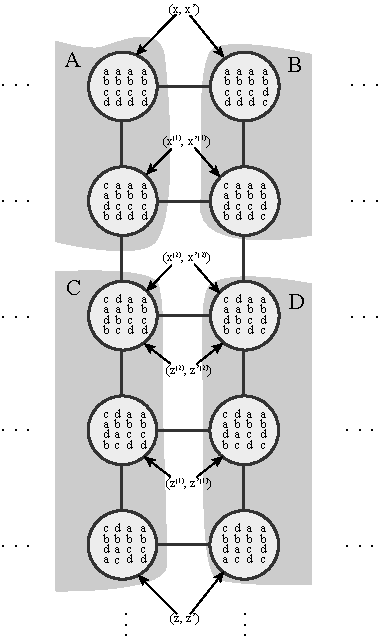
\includegraphics[width=5in]{../figures/diagram7.pdf}
			\caption{A visual example of a manipulation path.}
			\label{fig:manipulation-path}
		\end{center}
	\end{figure}


	We will now go through the example table step by step for the $x$ side (left half); the $z$ side is simply a mirror image of what happens in the $x$ side. At step 0 we have $x^{(0)} = x$ because we specified above that our initial value was $(x^{(0)}, x^{\prime(0)}) = (x,x')$. At step 1 we first use Equation \ref{eq:manipulation-path-rule-1-x} to essentially copy over every index from step 0 except index 1 (because it is the $k$\textsuperscript{th} index during this step). We then apply Equation \ref{eq:manipulation-path-rule-2-x} to index 1 to get $y_1$. At step 2 we again use Equation \ref{eq:manipulation-path-rule-1-x} to copy over every index from step 1 except for index 2 for which we use Equation \ref{eq:manipulation-path-rule-2-x} to get $y_2$. We don't modify the last two indices because these are the only ones on which $x, x'$ and $z, z'$ differ: recall that $(x, x') \in B_{n-1}^{a,b}$ and $(z, z') \in B_{n}^{c,d}$.

	\begin{lemma}[Lemma 5.1 of Isaksson, Kindler, and Mossel]
		For any SCF $f$, distinct $i, j \in \{1, \ldots, n\}$ and distinct alternatives $a, b, c, d \in C$ there exists a mapping $h : B_i^{a,b}(f) \times B_j^{c,d}(f) \rightarrow M$ where
		\[
			M = \{x \in P \mid f \text{ is manipulable at x}\}
		\]
		such that for any $x \in M$
		\[
			|h^{-1}(x)| \le 2n(m!)^{n+4}
		\]
	\end{lemma}
	\begin{proof}
		Without loss of generality, let $i = n - 1$ and $j = n$. We construct a manipulation path between $(x, x') \in B_i^{a,b}(f)$ and $(z, z') \in B_j^{c,d}(f)$. Notice that $(x, x')$ takes the values $(a, b)$ while $(z, z')$ takes the values $(c, d)$ because $f(x) = a$, $f(x') = b$, $f(z) = c$, and $f(z') = d$. Our claim is that along this manipulation path is an edge $(u, u'), (v, v')$ such that either
		\begin{enumerate}
			\item at least one of $u, u', v, v'$ is a manipulation point
			\item $f$ takes on at least three values on the points $u, u', v, v'$.
		\end{enumerate}
		In explanation, notice that there are at most three possible situations, and at least one of the above claims holds for each:
		\begin{itemize}
			\item On the first half of the path the value of the pair changes from $(a, b)$ to something else. If the first value changes to $b$ or the second value changes to $a$ then we have a manipulation point because the ranking of $a, b$ doesn't change on the first half of the path. Otherwise the values change to something other than $a$ or $b$, so $f$ takes at least three values at this point.
			\item On the second half of the path the value of the pair changes from $(c, d)$ to something else --- moving from the end towards the middle. If the first value changes to $d$ or the second value changes to $c$ then we have a manipulation point because the ranking of $c, d$ doesn't change on the second half of the path. Otherwise the values change to something other than $c$ or $d$, so $f$ takes at least three values at this point.
			\item The middle edge $(x^{(n-2)}, x^{\prime(n-2)}), (z^{(n-2)}, z^{\prime(n-2)})$ connects a pair with values $(a, b)$ and $(c, d)$. Clearly $f$ takes on at least three values at this point.
		\end{itemize}

		Notice that $u, u', v, v'$ agree in all but two indices which will be either $\{n - 1, k\}$, $\{n, k\}$, or $\{n - 1, n\}$ depending on whether $(u, u'), (v, v')$ is on the first half, on the second half, or is the middle edge of the path respectively. For example, if $(u, u'), (v, v')$ is on the first half of the path $u, u'$ and $v, v'$ will both differ on the $n - 1$ index because both pairs are in $B^{a,b}_{n-1}$. Additionaly, $u, v$ and $u', v'$ will each differ on $k$\textsuperscript{th} index because of the definition of the manipulation path.

		We claim that there exists a manipulation point $h((x, x'), (z, z')) = y$ which only differs from $u, u', v, v'$ on two indices. If Case 1 above holds, then we can let $y$ be whichever one of $u, u', v, v'$ is a manipulation point.

		If Case 2 holds then we apply the Gibbard-Satterthwaite to a restricted version of $f$, which we will call $f'$, which is $f$ restricted to the two indices on which $u, u', v, v'$ differ. We call these indices $k, p$. First we define a mapping $g : L(C)^2 \rightarrow L(C)^n$ which maps profiles from $f'$ to $f$.
		\begin{align*}
			g(x)_q &= u_q \,\,\, \forall q \notin \{k, p\} \\
			g(x)_k &= x_1 \\
			g(x)_p &= x_2.
		\end{align*}
		We define the set of alternatives to be $C$ where $|C| = m$ and we define $f' : L(C)^2 \rightarrow C$ such that
		\[
			f'(x) = f(g(x)).
		\]
		If we apply the Gibbard-Satterthwaite theorem \cite{gibbard1973manipulation, satterthwaite1975strategy} to $f'$ we will see that $f'$ is manipulable since it is not a dictator and it takes on at least 3 values (because Case 2 holds). Therefore some $x$ is a manipulation point for $f'$, so $g(x)$ is a manipulation point of $f$. And in fact $g(x)$ differs from $u, u', v, v'$ on only two indices so $y = g(x)$.

		The final step in the proof is to count the maximum number of pairs that could have lead to the manipulation point $y$ and that will be simply the number of inverses of the mapping function: $|h^{-1}(f)|$. To begin with, we know that the length of the manipulation path between $(x, x')$ and $(z, z')$ is $2n - 3$. This gives us $2n - 3$ possibilities for $(u, u'), (v, v')$. In addition, given $y$ there are at most $(q!)^2$ possibilities for $u$ because it differs from $y$ on at most two indices. We find that there are at most $(q!)^n$ possibilities for $x$ and $z$ as follows. For any $k \in \{1, \ldots, n\}$ we will have either:
		\begin{itemize}
			\item $u_k = x_k$ if $u$ is on the first half of the path and $k$ is an index that hasn't been updated --- by update we mean that it has been made to conform to $x_k =_{\{a,b\}} u_k =_{\overline{\{a,b\}}} z_k$. In this case there are $q!$ possibilities for $z_k$ because it can be any preference list.
			\item $u_k = z_k$ if $u$ is on the second half of the path and $k$ is an index that hasn't been updated. In this case there are $q!$ possibilities for $x_k$ because it can be any preference list.
			\item $x_k =_{\{a,b\}} u_k =_{\overline{\{a,b\}}} z_k$ if $k$ is an index that has been updated. In this case there are $\frac{q!}{2}$ possibilities for $x_k$ because only the order of $a, b$ needs to match $u_k$, and there are $2$ possibilities for $z_k$ because the order of every alternative besides $a, b$ needs to match $u_k$.
		\end{itemize}
		No matter which of the previous cases hold for each $k$, the total number of possibilities for $x$ and $z$ is still bounded above by $(q!)^n$.

		Lastly, given $x$ and $z$ there are at most $q!$ possibilitites for each of $x'$ and $z'$ respectively, since edges of the border set differ only in one index. Summing these we get:
		\begin{align*}
			|h^{-1}| &\le (2n - 3)(q!)^2(q!)^n(q!)(q!) \\
			|h^{-1}| &\le (2n - 3)(q!)^{n+4}.
		\end{align*}

	\end{proof}

	One of the open problems of Friedgut, Kalai, and Nisan was finding a way ``to replace the neutrality condition with the weaker `correct' condition: being far from having a range of size at most 2. \cite{friedgut2008elections}'' In 2011, Friedgut et al. successfully achieved this themselves with the help of one additional author \cite{friedgut2011quantitative}. Most of the work required to replace the neutrality condition focuses on the first step of the original theorem, and their results are as follows.
	\begin{theorem}
		There exist universal constants $C, C' > 0$ such that for every $\epsilon > 0$ and any $n$ the following holds:
		\begin{itemize}
			\item If $F$ is an SCF on $n$ voters and three alternatives, such that the distance of $F$ from a dictatorship and from having only two alternatives in its range is at least $\epsilon$, then
			\[
				\sum_{i=1}^n M_i(F) \ge C \cdot \epsilon^6.
			\]
			\item If, in addition, $F$ is neutral (that is, invariant under permutation of the alternatives), then:
			\[
				\sum_{i=1}^n M_i(F) \ge C' \cdot \epsilon^2.
			\]
		\end{itemize}
	\end{theorem}

	Mossel and R\'{a}cz \cite{mossel2011quantitative} took ideas from these two proofs and created a unified proof with the same results as Isaksson, Kindler, and Mossel, but without the neutrality constraint. This is a very useful result is as follows.
	\begin{theorem}
		Suppose we have $n \ge 1$ voters, $m \ge 3$ alternatives, and a SCF $f : L(C)^n \rightarrow C$ satisfying $\mathbf{D}(f, \mathrm{NONMANIP}) \ge \epsilon$. Then
		\[
			\mathbb{P}(\sigma \in M(f)) \ge \mathbb{P}(\sigma \in M_4(f)) \ge p \left( \epsilon, \frac{1}{n}, \frac{1}{m} \right)
		\]
		for some polynomial $p$, where $\sigma \in L(C)^n$ is selected uniformly. In particular, we show a lower bound of $\frac{\epsilon^{15}}{10^{39} n^{67} m^{166}}$.

		An immediate consequence is that
		\[
			\mathbb{P}((\sigma, \sigma') \text{ is a manipulation pair for } f) \ge q \left( \epsilon, \frac{1}{n}, \frac{1}{m} \right)
		\]
		for some polynomial $q$, where $\sigma \in L(C)^n$ is uniformly selected, and $\sigma'$ is obtained from $\sigma$ by uniformly selecting a coordinate $i \in \{ 1, \ldots, n \}$, uniformly selecting $j \in \{ 1, \ldots, n-3 \}$, and then uniformly randomly permuting the following four adjacent alternatives in $\sigma_i: \sigma_i(j), \sigma_i(j+1), \sigma_i(j+2),$ and $\sigma_i(j+3)$. In particular, the specific lower bound for $\mathbb{P}(\sigma \in M_4(f))$ implies that we can take $q \left( \epsilon, \frac{1}{n}, \frac{1}{m} \right) = \frac{\epsilon^{15}}{10^{41} n^{68} m^{167}}$.
	\end{theorem}

	Above the distance between SCFs is defined to be the fraction of inputs on which they differ: $\mathbf{D}(f, g) = \mathbb{P}(f (\sigma) \ne g(\sigma))$, and for a class of SCFs $G$ we take the SCF with the minimum distance: $\mathbf{D}(f, G) = \min_{g \in G} \mathbf{D}(f, g)$. NONMANIP is defined to be the set of SCFs which are either dictators or take at most two values. Finally, $M(f)$ denotes the set of manipulation points of the SCF f, and for a given $r$, let $M_r(f)$ denote the set of $r$-manipulation points of $f$ (we only allow permuting $r$ adjacent alternatives instead of the entire preference list).

%!TEX root = thesis.tex

\chapter{Results}

	In this chapter we will attempt to generalize step 3 of Friedgut by way of generalizing Friedgut's Lemma 6, Lemma 7, and Lemma 8. However, we will begin the chapter with some general lattice theory results that we will need later on in the chapter.

\section{Lattice Theory}

	We are not aware of any existing proofs of these lemmas, but some of them are fairly elementary and have a broad application, so they could have previously been proven by others.

	First we will prove, in three steps, that our inversion lattice (ordered by $\le_s$; Definition \ref{partial-order-s-definition}) remains a lattice when we enforce an order between two neighboring elements in the order (Definition \ref{identified-lattice-definition}). Recall from Definition \ref{lattice-definition} that in order to be a lattice the join and meet must exist for every pair of elements. Therefore Lemma \ref{identified-permutation-lattice-join} proves that the join exists, Lemma \ref{identified-permutation-lattice-meet} proves that the meet exists (with similar reasoning), and Proposition \ref{proposition-identification-is-lattice} combines both lemmas to prove that our structure is indeed still a lattice.

	\begin{lemma}
		\label{identified-permutation-lattice-join}
		Let $(Y, \le)$ be a poset and let $X = S(Y)$. Let $(X, \le_s)$ as in Definition \ref{partial-order-s-definition}. Let $\Inv$ be the inversion binary relation (Definition \ref{inversion-definition}) over $Y$, and let $\join$ and $\join^{ij}$ denote the join in $(X, \le_s)$ and $(X^{ij}, \le^{ij}_s)$ respectively. Then for any $i,j \in Y$, if $i$ is either a direct successor or a direct predecessor of $j$ according to $\le_s$, it holds that for all $x, y \in X^{ij}$:
		\[
			x \join y \text{ is defined} \implies x \join^{ij} y \text{ is defined}.
		\]
	\end{lemma}

	\begin{proof}
		Assume $x \join y$ is defined. Let $z = x \join y$. Then $z$ is an upper bound of $\{x, y\}$:
		\[
			z \ge_s x \textrm{ and } z \ge_s y.
		\]
		And $z$ is the least upper bound of $\{x, y\}$. For every $a \in X$:
		\[
			(a \ge_s x \textrm{ and } a \ge_s y) \implies z \le_s a.
		\]
		Since $x \in X^{ij}$, then $(i, j) \notin Inv_x$. Since $z \ge_s x$, then $(i, j) \notin Inv_z$, so $z \in X^{ij}$. By definition $z \ge_s x \implies z \ge^{ij}_s x$ and $z \ge_s y \implies z \ge^{ij}_s y$. Therefore $z$ is an upper bound of $\{x, y\}$ in $X^{ij}$.

		For any $a \in X^{ij}$ if $a$ is an upper bound of $\{x, y\}$ in $X^{ij}$ then clearly $a$ is also an upper bound of $\{x, y\}$ in $X$. Therefore $z \le_s a$, so $z \le^{ij}_s a$, which means $z = x \join^{ij} y$. So clearly $x \join^{ij} y$ exists.
	\end{proof}

	\begin{lemma}
		\label{identified-permutation-lattice-meet}
		Let $Y$ be a set and let $X = S(Y)$. Let $(X, \le_s)$ be a lattice with $\le_s$ defined as above. Let $\Inv$ be the inversion binary relation over $Y$ as defined above. Let $\meet$ and $\meet^{ij}$ denote the meet in $(X, \le_s)$ and $(X^{ij}, \le^{ij}_s)$ respectively. Then for any $i,j \in Y$, if $i$ is either a direct successor or a direct predecessor of $j$ according to $\le_s$, it holds that for all $x, y \in X^{ij}$:
		\[
			x \meet y \text{ is defined} \implies x \meet^{ij} y \text{ is defined}.
		\]
	\end{lemma}

	\begin{proof}
		Assume $x \meet y$ is defined. Let $z = x \meet y$. Then $z$ is a lower bound of $\{x, y\}$:
		\[
			z \le_s x \textrm{ and } z \le_s y.
		\]
		And $z$ is the greatest lower bound of $\{x, y\}$: for every $a \in X$:
		\[
			(a \le_s x \textrm{ and } a \le_s y) \implies z \ge_s a.
		\]
		We now show that $z \in X^{ij}$. Since $z = x \meet y$, it holds that $\Inv_z = (\Inv_x \cup \Inv_y)^t$ (Definition \ref{transitive-closure-definition}, Definition \ref{partial-order-s-definition}) \cite{markowsky1994permutation}. Because $x,y \in X^{ij}$ we know that $(i, j) \notin (\Inv_x \cup \Inv_y)$. Therefore, in order to have $(i, j) \in (\Inv_x \cup \Inv_y)^t$ we would need to have $(i, k) \in \Inv_x$ and $(k, j) \in \Inv_y$ for some $k \in Y$, which is impossible because $i$ is either a direct successor or a direct predecessor of $j$. Therefore $(i, j) \notin Inv_z$, so $z \in X^{ij}$.

		By definition $z \le_s x \implies z \le^{ij}_s x$ and $z \le_s y \implies z \le^{ij}_s y$. Therefore $z$ is a lower bound of $\{x, y\}$ in $X^{ij}$.

		For any $a \in X^{ij}$ if $a$ is a lower bound of $\{x, y\}$ in $X^{ij}$ then clearly $a$ is also a lower bound of $\{x, y\}$ in $X$. Therefore $z \ge_s a$, so $z \ge^{ij}_s a$, which means $z = x \meet^{ij} y$. So clearly $x \meet^{ij} y$ is defined.
	\end{proof}

	\begin{proposition}
		\label{proposition-identification-is-lattice}
		Let $Y$ be a set and let $X = S(Y)$. Let $(X, \le_s)$ be a lattice with $\le_s$ defined as above. Let $\Inv$ be the inversion binary relation over $Y$ as defined above. Then for any $i,j \in Y$, if $i$ is either a direct successor or a direct predecessor of $j$ according to $\le_s$, it holds that $(X^{ij}, \le^{ij}_s)$ is a lattice.
	\end{proposition}

	\begin{proof}
		We know that $x \join y$ is defined and $x \meet y$ is defined because $(X, \le_s)$ is a lattice. Therefore by Lemma \ref{identified-permutation-lattice-join} and Lemma \ref{identified-permutation-lattice-meet} we have $x \join^{ij} y$ is defined and $x \meet^{ij} y$ is defined respectively. So $(X^{ij}, \le^{ij}_s)$ is a lattice, by definition of a lattice.
	\end{proof}

	Now we will show that a cross-product of lattices is also a lattice. For example, suppose we have the lattice in Figure \ref{figure-one-dimensional-lattice}. The top element is the greatest, and the arrows show the ``less than'' relationship between elements. Each column of numbers represents a ranking of alternatives ${1, 2, 3}$ in which we don't care about the relationship between alternative $1$ and $2$ so we simply replace alternative $2$ with $1$ in the ranking. All this aside though, this proof is valid for any lattice.

	\begin{figure}[ht]
		\begin{center}
			\includegraphics[width=1in]{../figures/diagram5.pdf}
			\caption{A single dimension of lattice.}
			\label{figure-one-dimensional-lattice}
		\end{center}
	\end{figure}

	If we were to make that lattice into a 2-dimensional ``grid'' it would look like Figure \ref{figure-two-dimensional-lattice}. This would be the case if we only had two voters ($n = 2$).

	\begin{figure}[ht]
		\begin{center}
			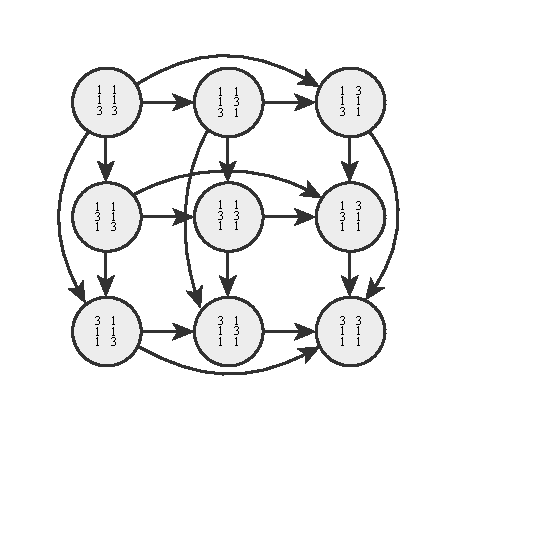
\includegraphics[width=3in]{../figures/diagram6.pdf}
			\caption{A 2-dimensional version of the lattice from Figure \ref{figure-one-dimensional-lattice}.}
			\label{figure-two-dimensional-lattice}
		\end{center}
	\end{figure}

	\begin{proposition}
		\label{proposition-grid-is-lattice}
		Let $(X, \le)$ be a lattice. Let $X^n$ be the set of all $n$-tuples of elements of $X$. Let $\le^n$ be defined as: for all $x, y \in X$
		\[
			x \le^n y \iff \forall i \in \{1, \ldots, n\}, x_i \le y_i.
		\]
		Then $(X^n, \le^n)$ is a lattice.
	\end{proposition}

	\begin{proof}
		By definition of a lattice, $(X^n, \le^n)$ is a lattice if for any two elements $s, t \in S^n$, $s \join t$ is defined and $s \meet t$ is defined.

		First, we show that $s \join t$ is defined. We define $u \in X^n$ such that $u_i = s_i \join t_i$, $\forall i \in \{1, \ldots, n\}$, and we show that $u = s \join t$. Because $u_i = s_i \join t_i$, we have
		\[
			u_i \ge s_i \textrm{ and } u_i \ge s_i
		\]
		so
		\[
			u \ge^n s \textrm{ and } u \ge^n t
		\]
		meaning that $u$ is an upper bound for $s$ and $t$. Suppose there is some $v \in X^n$ which is also an upper bound for $s$ and $t$. Then $\forall i \in \{1, \ldots, n\}$ we have
		\[
			v_i \ge s_i \textrm{ and } v_i \ge t_i
		\]
		so since $u_i = s_i \join t_i$, then $u_i \le v_i$. Therefore $u \le^n v$, i.e. $u$ is the least upper bound of $\{s, t\}$.

		Second, it follows by analogy to the above proof for $s \join t$, that $s \meet t$ is defined. Therefore, $s \join t$ is defined and $s \meet t$ is defined, so $(X^n, \le^n)$ is a lattice.
	\end{proof}


\section{Main Theorem}

	Hereafter, since we refer very often to \cite{friedgut2008elections}, instead of saying for example ``Lemma 2 of Friedgut, Kalai, and Nisan'' we will often shorten it to ``Lemma 2 Friedgut''.

	Friedgut, Kalai, and Nisan's main theorem is proved in three steps; the first two are already general, and hold for any $n, m \in N^+$. Therefore, to generalize the main theorem we need only generalize the third step, and therefore this third step is our main theorem. This step is comprised of Lemma 6, Lemma 7, and Lemma 8 which we will generalize one at a time. The lemma we will generalize is:

	\begin{lemma}[Lemma 3 of Friedgut]
		For every SCF $f$ on $3$ alternatives and every $a,b \in A$,
		\[
			M^{a,b} \le \sum_i M_i \cdot 6
		\]
	\end{lemma}

	Which we will generalize as:

	\begin{theorem}[Main Theorem]
		For every SCF $f$ on $m$ alternatives and every $a, b \in C$:
		\[
			M^{a, b}(f) \le m! \cdot \sum_i M_i(f)
		\]
	\end{theorem}

	For the rest of the proof we will fix a SCF, $f$, and two alternatives $a, b \in C$.


\section{Generalized Lemma 6 of Friedgut}

	For any preference profile $p \in P$ there are $(\frac{m!}{2})^n$ profiles $x$ such that $x|_{\{a, b\}} = p|_{\{a, b\}}$. This is because there are $m!$ possible preference lists; half of them will have the preference between $a$ and $b$ that agrees with $p|_{\{a, b\}}$ and half will disagree. This gives $\frac{m!}{2}$ possible preference lists for each voter, so there are $(\frac{m!}{2})^n$ profiles comprised of these preference lists.

	\begin{definition}
		Let $a, b \in C$ be the first two alternatives, let $p \in L(C)^n$ be a preference profile, and let $X \subseteq L(C)^n$. We define
		\begin{align*}
			A(p, X) &= \{x \in X \mid x|_{\{a,b\}} = p|_{\{a,b\}}, f(x) = a\} \\
			B(p, X) &= \{x \in X \mid x|_{\{a,b\}} = p|_{\{a,b\}}, f(x) = b\}.
		\end{align*}
		When we do not explicitly specify $X$ we assume $X = L(C)^n$:
		\begin{align*}
			A(p) &= A(p, L(C)^n) \\
			B(p) &= B(p, L(C)^n).
		\end{align*}
	\end{definition}

	Before we state Lemma \ref{friedgut-lemma-6}, recall the definition of $M^{a,b}(f)$ from Friedgut \cite{friedgut2008elections}:
	\[
		M^{a,b}(f) = \probability(f(p) = a, f(p') = b)
	\]
	where $p, p'$ are chosen at random in $L(C)^n$ with $p|_{\{a,b\}} = p'|_{\{a,b\}}$.

	Therefore we can rewrite $M^{a,b}(f)$ as follows.

	\begin{lemma}[Lemma 6 of Friedgut]
		\label{friedgut-lemma-6}
		\[
			M^{a,b}(f) = E_{q \in L(C)^n} \left[ \frac{|A(q)|}{\left(\frac{m!}{2}\right)^n} \cdot \frac{|B(q)|}{\left(\frac{m!}{2}\right)^n} \right]
		\]
	\end{lemma}
	\begin{proof}
		First we fix a profile $q$. Then
		\[
			\frac{|A(q)|}{\left(\frac{m!}{2}\right)^n}
		\]
		is the probability that a randomly chosen profile, $p$, satisfying $p|_{\{a,b\}} = q|_{\{a,b\}}$ also satisfies $f(p) = a$. This is because there are $(\frac{m!}{2})^n$ profiles that agree with $q|_{\{a,b\}}$, and $|A(q)|$ is the number of those for which the outcome is $a$.

		Likewise,
		\[
			\frac{|B(q)|}{\left(\frac{m!}{2}\right)^n}
		\]
		is the probability that a randomly chosen profile, $p'$, satisfying $p'|_{\{a,b\}} = q|_{\{a,b\}}$ also satisfies $f(p') = b$.

		Since $p|_{\{a,b\}} = q|_{\{a,b\}}$ and $p'|_{\{a,b\}} = q|_{\{a,b\}}$, clearly we have that $p|_{\{a,b\}} = p'|_{\{a,b\}}$. Since $f(p) = a$ and $f(p') = b$ are independent events, the joint probability is
		\[
			\frac{|A(q)|}{\left(\frac{m!}{2}\right)^n} \cdot \frac{|B(q)|}{\left(\frac{m!}{2}\right)^n}.
		\]
	\end{proof}


\section{Generalized Lemma 7 of Friedgut}

	We now attempt to relate $M_i(f)$ to $A$ and $B$.

	Recall the ordering, $\le_s$, which was defined in Definition \ref{partial-order-s-definition}. We know that $(L(C), \le_s)$ is a lattice by the following. First, $L(C)$ is the set of all total orderings of $C$, which is isomorphic to the set of all permutations of $C$. Second, $\le_s$ is the weak Bruhat order (also known as the weak order of permutations). The weak Bruhat order applied to the set of all permutations is a lattice \cite{bjorner1984orderings}, so $(L(C), \le_s)$ is a lattice. This is useful to note now, and will be invoked to help prove Lemma \ref{friedgut-lemma-8}.

	We have defined $(L(C), \le_s)$ to be a lattice, but for the following definition, and for later in the chapter we will treat it as a graph with $L(C)$ being the set of vertices, and $\le_s$ being the set of edges.

	\begin{definition}
		Let $p \in L(C)^n$. We define the \emph{upper edge border} of $A(p)$, denoted $\partial A(p)$, to be the set of directed edges whose tail is in $A(p)$ and whose head is not in $A(p)$. We will use the notation $(x_{-i}, x_i, x'_i)$ as a shorthand to denote the edge $((x_{-i},x_i), (x_{-i},x'_i))$. Formally, for all $i \in \{1, \ldots, n\}$:
			\begin{align*}
				\partial_i A(p) = \{ (x_{-i}, x_i, x'_i) \mid \hspace{1mm} & (x_{-i}, x_i) \in A(p), \\
				& (x_{-i}, x'_i) \notin A(p), \\
				& x_i|_{\{a,b\}} = x'_i|_{\{a,b\}}, \\
				& x_i <_s x'_i \}
			\end{align*}
		and
			\[
				\partial A(p) = \bigcup_j \partial_j A(p)
			\]
		We define the upper edge border of $B(p)$ analogously.
	\end{definition}

	\begin{lemma}
		\label{manipulation-per-edge-in-a}
		Let $p, p' \in L(C)^n$, and let $i \in \{1, \ldots, n\}$. Let the following conditions hold:
		\begin{align*}
			p_{-i} &= p'_{-i} \\
			p_i|_{a,b} &= p'_i|_{a,b}.
		\end{align*}
		Then each $(x_{-i}, x_i, x'_i) \in \partial_i A(p) \cup \partial_i B(p)$ corresponds to at least one successful manipulation.
	\end{lemma}

	\begin{proof}
		By definition of the upper edge border we have
		\begin{align*}
			x_i &<_s x'_i \text{ and} \\
			x_i|_{\{a,b\}} &= x'_i|_{\{a,b\}}.
		\end{align*}

		For $(x_{-i}, x_i, x'_i) \in \partial_i A(p)$, we know that $f((x_{-i}, x_i)) = a$ and $f((x_{-i}, x'_i)) = t$ for $t \in C \backslash \{a\}$. If $t \succ_{x_i} a$ then $x'_i$ is a successful manipulation of $(x_{-i}, x_i)$. Otherwise, $a \succ_{x_i} t$. If this is the case, then we know that $(a, t) \notin Inv_{x_i}$, and because $x_i <_s x'_i$ we have $(a, t) \notin Inv_{x'_i}$, which means $a \succ_{x'_i} t$. Therefore $x_i$ is a successful manipulation of $(x_{-i}, x'_i)$.

		And analogously for $(x_{-i}, x_i, x'_i) \in \partial_i B(p)$, either $x'_i$ is a successful manipulation of $(x_{-i}, x_i)$ or $x_i$ is a successful manipulation of $(x_{-i}, x'_i)$.
	\end{proof}

	We now generalize Lemma 7 of Friedgut, Kalait, and Nisan. Their original lemma is:

	\begin{lemma}[Lemma 7 of Friedgut]
		\[
			M_i(f) \ge \frac{1}{6} 3^{-n} E_x \left[|\partial_i A(p)| + |\partial_i B(p)| \right]
		\]
	\end{lemma}

	And we generalize it as follows.

	\begin{lemma}
		\label{friedgut-lemma-7}
		\[
			M_i(f) \ge \frac{1}{m!} \left(\frac{m!}{2}\right)^{-n} E_x \left[|\partial_i A(p)| + |\partial_i B(p)| \right]
		\]
	\end{lemma}

	\begin{proof}
		Recall the definition of $M_i(f)$: given a profile $p \in P$ and a vote $p'_i \in V$ chosen uniformly at random, $M_i(f)$ is the probability that $p'_i$ is a successful manipulation of $p$ by voter $i$. Therefore to lower bound $M_i(f)$ we start with $p$ and $p'_i$ chosen uniformly at random. We can think of these as two distinct profiles, $p$ and $p'$, where $p' = (p_{-i}, p'_i)$.

		Clearly $p_{-i}|_{\{a,b\}} = p'_{-i}|_{\{a,b\}}$, but we will have $p_i|_{\{a,b\}} = p'_i|_{\{a,b\}}$ only with probability $\frac{1}{2}$, and we condition the following on this being the case. So we assume that $p|_{\{a,b\}} = p'|_{\{a,b\}}$.

		By Lemma \ref{manipulation-per-edge-in-a}, each $(x_{-i}, x_i, x'_i) \in (\partial_i A(p) \cup \partial_i B(p))$ corresponds to at least one successful manipulation. Note that if $(x_{-i}, x_i, x'_i) \in \partial_i A(p)$ then $(x_{-i}, x'_i, x_i) \notin \partial_i A(p)$.

		We take a short aside to limit our domain without losing any information. Since we have conditioned this line of reasoning such that $p|_{\{a,b\}} = p'|_{\{a,b\}}$, for any two votes $v_1, v_2 \in A(p) \cup B(p) \cup A(p') \cup B(p')$ we have $v_1|_{\{a,b\}} = v_2|_{\{a,b\}}$. Therefore we can define a new set
		\[
			P' = \{x \in L(C)^n \mid x|_{\{a,b\}} = p|_{\{a,b\}}\}
		\]
		and view $A(p), B(p)$, as residing in $P'$. This is because, by definition, the elements of these sets agree with $p|_{\{a,b\}}$. Clearly $|P'| = (\frac{m!}{2})^n$.

		Therefore we can lower bound $M_i(f)$ by the probability that an edge is in either $\partial_i A(p)$ or $\partial_i B(p)$. The total possible number of edges is
		\[
			\frac{m!}{2} \cdot \frac{m!}{2} \cdot \left(\frac{m!}{2}\right)^{n-1} = \frac{m!}{2}\left(\frac{m!}{2}\right)^{n}
		\]
		So the probability that a randomly chosen edge is in either $\partial_i A(p)$ or $\partial_i B(p)$ is
		\[
			\frac{2}{m!} \left(\frac{2}{m!}\right)^{n} \cdot E \left[ |\partial_i A(p)| + |\partial_i B(p)| \right]
		\]
		Note that we can sum the probabilities for $\partial_i A(p)$ and $\partial_i B(p)$ because they are disjoint by the definition of the upper edge border; an edge cannot satisfy both $(x_{-i}, x_i) \in A(p)$ and $(x_{-i}, x_i) \in B(p)$ simultaneously because if $f((x_{-i}, x_i)) = a$ then $f((x_{-i}, x_i)) \ne b$ and vice versa.

		We conditioned our analysis on $p_{-i}|_{\{a,b\}} = p'_{-i}|_{\{a,b\}}$, so our lower bound becomes
		\[
			M_i(f) \ge \frac{1}{2} \cdot \frac{2}{m!}\left(\frac{2}{m!}\right)^{n} \cdot E \left[ |\partial_i A(p)| + |\partial_i B(p)| \right].
		\]
		After simplifying, we have
		\[
			M_i(f) \ge \frac{1}{m!}\left(\frac{2}{m!}\right)^{n} \cdot E \left[ |\partial_i A(p)| + |\partial_i B(p)| \right].
		\]
	\end{proof}

	Summing over $i$ we get the following corollary.

	\begin{corollary}[Corollary 1 of Friedgut]
		\[
			\frac{1}{m!} \cdot \left(\frac{m!}{2}\right)^{-n} E_p[|\partial A(p)| + |\partial B(p)|] \le \sum_i M_i(f)
		\]
	\end{corollary}


\section{Generalized Lemma 8 of Friedgut}

	In this section we will fix a profile $p$, and for the sake of readability we use the following shorthand notation:
	\begin{align*}
		\le^n &\equiv (\le_s)^n \\
		A &\equiv A(p) \\
		B &\equiv B(p) \\
		A(X) &\equiv A(p, X) \\
		B(X) &\equiv B(p, X).
	\end{align*}
	We also recall $(L(C)^n, \le^n)$ is our $n$-dimensional lattice, and that $A$ and $B$ reside in this space:
	\begin{align*}
		A &\subseteq L(C)^n \\
		B &\subseteq L(C)^n \\
	\end{align*}

	We now generalize Lemma 8 of Friedgut, Kalait, and Nisan. Their original lemma is:

	\begin{lemma}[Lemma 8 of Freidgut]
		For every disjoint $A, B$ we have that
		\[
			|\partial A| + |\partial B| \ge \left( \frac{1}{3} \right)^n |A| \cdot |B|
		\]
	\end{lemma}

	Our generalization of the above lemma is Lemma \ref{friedgut-lemma-8}, but we must do a little bit of setup before we are ready to prove it. First we define an algorithm to consolidate $A$ into $A'$. We define $A'$ to be a consolidation of $A$ as follows. Let $A' = \emptyset$.

	\begin{algorithm}
		\begin{algorithmic}
			\For{$i = 1 \to n$}
				\For{$d \in L(C)^n$}
					\State $D \gets \{x \in L(C)^n \mid x_{-i} = d_{-i}\}$
					\For{$a \in A(D)$}
						\State $a' \gets \max_{\le^n}(A(D) \backslash A')$
						\State $A' \gets A' \cup \{a'\}$
					\EndFor
				\EndFor
			\EndFor
		\end{algorithmic}
	\end{algorithm}

	We do the same to consolidate $B$ into $B'$.

	For each $D$ above, we now have that either $A'(D) \subseteq B'(D)$ or $B'(D) \subseteq A'(D)$. Unfortunately, we need $A' \subseteq B'$ or $B' \subseteq A'$ which does not necessarily follow; see Open Problem \ref{lemma-8-open-problem}.

	\begin{openproblem}
		\label{lemma-8-open-problem}
		When using the algorithm above, we do not necessarily have $A' \subseteq B'$ or $B' \subseteq A'$. We could probably fix this by changing:
		\[
			a' \gets \max_{\le^n}(A(D) \backslash A')
		\]
		to something like
		\[
			a' \gets \max_{\le^n}(A \backslash A')
		\]
		but then it becomes difficult to prove
		\begin{align*}
			|A' \backslash A| &\le |\partial A| \textrm{ and} \\
			|B' \backslash B| &\le |\partial B|.
		\end{align*}
		Therefore, we leave this as our first open problem.

		We will continue with the proof as if we do have $A' \subseteq B'$ or $B' \subseteq A'$, so that if this problem is resolved then the proof will be complete.
	\end{openproblem}

	We will now prove the following lemma.
	\begin{lemma}
		\label{lemma-8-enough-edges}
		\begin{align*}
			|A' \backslash A| &\le |\partial A| \textrm{ and} \\
			|B' \backslash B| &\le |\partial B| \\
		\end{align*}
	\end{lemma}

	\begin{proof}
		First, we show that for every $a' \in A' \backslash A$, we have an edge in $\partial A$.

		Let $a' \in A' \backslash A$. The above algorithm only adds elements to $A'$ in the innermost for loop, and since that for loop iterates once for every $a \in A(D)$ we know that for every $a'$ we have a corresponding $a$. Since $a' \in A' \backslash A$, we know that $a \ne a'$. Since $a' \gets \max_{\le^n}(A(D) \backslash A')$ and $a \ne a'$, we have that $a <^n a'$. According to the algorithm, $a, a' \in D$ which means $a_{-i} = a'_{-i}$. Therefore, $(a_{-i}, a_i, a'_i) \in \partial_i A$ by the definition of $\partial_i A$.

		Therefore, every profile in $A' \backslash A$ corresponds to at least one profile in $\partial A$, so we know that
		\[
			|A' \backslash A| \le |\partial A|.
		\]
		The same reasoning can be used to show that:
		\[
			|B' \backslash B| \le |\partial B|.
		\]
	\end{proof}

	And now we are ready to prove the final lemma in this section:

	\begin{lemma}
		\label{friedgut-lemma-8}
		For every disjoint $A, B$ we have that
		\[
			|\partial A| + |\partial B| \ge \left( \frac{2}{m!} \right)^n |A| \cdot |B|
		\]
	\end{lemma}

	\begin{proof}
		Since for any two votes $v_1, v_2 \in A \cup B$ we have $v_1|_{\{a,b\}} = v_2|_{\{a,b\}}$ we can define a new set
		\[
			P' = \{x \in P \mid x|_{\{a,b\}} = p|_{\{a,b\}}\}
		\]
		and view $A$, $B$, $A'$, and $B'$ as residing in $P'$ without losing any information. This is because, by definition, the elements of these sets agree with $p|_{\{a,b\}}$. Clearly $|P'| = (\frac{m!}{2})^n$.

		For any vote $v \in P'$, let $E_{A'}$ be the event that $v$ is in $A'$, and let $E_{B'}$ be the event that $v$ is in $B'$. Then
		\[
			P(E_{A'} \cap E_{B'}) = P(E_{A'}) P(E_{B'}|E_{A'})
		\]
		Clearly
		\begin{align}
			\label{probability-values-1}
			P(E_{A'} \cap E_{B'}) &= \frac{|A' \cap B'|}{|P'|} \\
			\label{probability-values-2}
			P(E_{A'}) &= \frac{|A'|}{|P'|} \\
			\label{probability-values-3}
			P(E_{B'}) &= \frac{|B'|}{|P'|}
		\end{align}
		Since either $A' \subseteq B'$ or $B' \subseteq A'$, we have
		\[
			P(E_{B'}|E_{A'}) \ge P(E_{B'})
		\]
		Therefore
		\[
			P(E_A \cap E_B) \ge P(E_A) P(E_B)
		\]
		So by substitution from equations \ref{probability-values-1}, \ref{probability-values-2}, and \ref{probability-values-3} we get
		\begin{align*}
			\frac{|A' \cap B'|}{(\frac{m!}{2})^n} &\ge \frac{|A'|}{(\frac{m!}{2})^n} \frac{|B'|}{(\frac{m!}{2})^n} \\
			&= \frac{|A|}{(\frac{m!}{2})^n} \frac{|B|}{(\frac{m!}{2})^n}
		\end{align*}
		However $A$ and $B$ are disjoint so
		\[
			A' \cap B' \subseteq (A' \backslash A) \cup (B' \backslash B)
		\]
		which, along with Lemma \ref{lemma-8-enough-edges}, completes the proof as follows
		\begin{align*}
			|A' \cap B'| &\le |A' \backslash A| + |B' \backslash B| \\
			|A' \cap B'| &\le |\partial A| + |\partial B| \\
			\frac{|A||B|}{(\frac{m!}{2})^n} &\le |\partial A| + |\partial B| \\
			\left(\frac{2}{m!}\right)^n |A| \cdot |B| &\le |\partial A| + |\partial B| \\
			|\partial A| + |\partial B| &\ge \left(\frac{2}{m!}\right)^n |A| \cdot |B| \\
		\end{align*}
	\end{proof}

\section{Finished Step 3 of Friedgut}

	Lemma 6, 7, and 8 fit together as follows. First we define the variables $L_6$, $L_7$, and $L_8$ to be variable values that multiply each of the lemmas respectively. The values of these variables will change depending on the value of $m$, so we evaluate the lemmas in terms of these variables to be more general. We can define the lemmas in terms of these variables:
	\begin{align*}
		&M^{a,b} = E[|A||B|] \cdot L_6 & \textrm{lemma 6} \\
		&L_7 \cdot E[|\partial A| + |\partial B|] \le \sum_i M_i & \textrm{lemma 7} \\
		&\frac{1}{L_8} \cdot (|\partial A| + |\partial B|) \ge |A||B| & \textrm{lemma 8}
	\end{align*}

	Now we can solve for the result of step 3.
	\begin{align*}
		M^{a,b} &= E[|A||B|] \cdot L_6 & \textrm{by lemma 6} \\
		M^{a,b} &\le E[|\partial A| + |\partial B|] \cdot \frac{L_6}{L_8} & \textrm{by lemma 8} \\
		M^{a,b} &\le \sum_i M_i \cdot \frac{L_6}{L_7L_8} & \textrm{by lemma 7}
	\end{align*}

	If we can fully generalize this step and capture all of the $v_i$'s our results will, possibly, look like this:
	\begin{align*}
		L_6 &= \left(\frac{m!}{2}\right)^{-2n} \\
		L_7 &= \frac{1}{m!}\left(\frac{m!}{2}\right)^{-n} \\
		L_8 &= \left(\frac{m!}{2}\right)^{-n}
	\end{align*}

	So we have that
	\begin{align*}
		\frac{L_6}{L_7L_8} &= \left(\frac{m!}{2}\right)^{-2n} \cdot m!\left(\frac{m!}{2}\right)^{n} \cdot \left(\frac{m!}{2}\right)^{n} \\
		&= \left(\frac{m!}{2}\right)^{-2n} \cdot m! \cdot \left(\frac{m!}{2}\right)^{2n} \\
		&= m!
	\end{align*}

	And the final result for step 3 becomes
	\begin{align*}
		M^{a,b} &\le \sum_i M_i \cdot m!
	\end{align*}

\section{Main Theorem of Friedgut}

	Now we can use the Friedgut's generalized steps 1 and 2 along with our generalized version of step 3 to prove a general version of Friedgut's main theorem. We will restate Friedgut's generalized lemmas from step 1 and 2.

	\begin{lemma}[Lemma 1 of Friedgut]
		\label{friedgut-lemma-1}
		For every fixed $m$ and $\epsilon > 0$ there exists $\delta > 0$ such that if $F = f^{\otimes \binom{m}{2}}$ is a neutral IIA GSWF over $m$ alternatives with $f : \{0,1\}^n \rightarrow \{0,1\}$, and $\Delta(f, DICT) > \epsilon$, then $F$ has probability of at least $\delta \ge (C\epsilon)^{\lfloor m/3 \rfloor}$ of not having a Generalized Condorcet Winner, where $C > 0$ is an absolute constant.
	\end{lemma}

	\begin{lemma}[Lemma 2 of Friedgut]
		\label{friedgut-lemma-2}
		For every fixed $m$ there exists $\delta > 0$ such that for all $\epsilon > 0$ the following holds. Let $f$ be a neutral SCF among $m$ alternatives such that $\Delta(f, DICT) > \epsilon$. Then for all $(a,b)$ we have $M^{a,b}(f) \ge \delta$.
	\end{lemma}

	And we restate our generalized version of Friedgut's Lemma 3.

	\begin{lemma}[Lemma 3 of Friedgut]
		\label{friedgut-lemma-3}
		For every SCF $f$ on $m$ alternatives and every $a,b \in A$, $M^{a,b} \le \sum_i M_i \cdot m!$
	\end{lemma}

	With these three lemmas we can now prove a generalized version of Friedgut's main theorem.

	\begin{theorem}[Theorem 1 of Friedgut]
		There exists a constant $C > 0$ such that for every $\epsilon > 0$ the following holds. If $f$ is a neutral SCF for $n$ voters over 3 alternatives and $\Delta(f, g) > \epsilon$ for any dictatorship $g$, then $f$ has total manipulatiblity: $\sum^n_{i=1} M_i(f) \ge \frac{(C\epsilon)^{\lfloor m/3 \rfloor}}{m!}$.
	\end{theorem}

	\begin{proof}
		Lemma \ref{friedgut-lemma-2} gives us
		\begin{align*}
			M^{a,b}(f) \ge \delta
		\end{align*}
		and by substituting the result from Lemma \ref{friedgut-lemma-1} for $\delta$ we get
		\begin{align*}
			M^{a,b}(f) &\ge \delta \ge (C\epsilon)^{\lfloor m/3 \rfloor} \\
			M^{a,b}(f) &\ge (C\epsilon)^{\lfloor m/3 \rfloor} \\
		\end{align*}
		We then relate $M^{a,b}$ to $M_i$ by Lemma \ref{friedgut-lemma-3}
		\begin{align*}
			\sum^n_{i=1} M_i(f) \cdot m! &\ge M^{a,b}(f) \ge (C\epsilon)^{\lfloor m/3 \rfloor} \\
			\sum^n_{i=1} M_i(f) \cdot m! &\ge (C\epsilon)^{\lfloor m/3 \rfloor} \\
			\sum^n_{i=1} M_i(f) &\ge \frac{(C\epsilon)^{\lfloor m/3 \rfloor}}{m!} \\
		\end{align*}
	\end{proof}

%!TEX root = thesis.tex

\chapter{Conclusion}

	We have attempted to prove the following main result in order to extend the results of Friedgut, Kalai, and Nisan in a straightforward manner, and along the same lines of reasoning as the original proof. Our main theorem is

	\begin{theorem}[Main Result]
		There exists a constant $C > 0$ such that for every $\epsilon > 0$ the following holds. If $f$ is a neutral SCF for $n$ voters over 3 alternatives and $\Delta(f, g) > \epsilon$ for any dictatorship $g$, then $f$ has total manipulatiblity: $\sum^n_{i=1} M_i(f) \ge \frac{(C\epsilon)^{\lfloor m/3 \rfloor}}{m!}$.
	\end{theorem}

	Unfortunately, due to time constraints we were unable to prove (or disprove) Lemma \ref{friedgut-lemma-8} because of the problem noted in the attempted proof for that lemma. We conjecture that this can be proven without many changes to our attempted proof, and we leave this as our first open problem.

	Since our main result relies on Lemma \ref{friedgut-lemma-8}, we have only been able to show the following two lemmas.

	\begin{lemma}
		Let $C$ be a set of alternatives. Let $a, b \in C$ be any two alternatives. Let $m = |C|$ and let $n$ be the number of voters. Let $f$ be a SCF. We have
		\[
			M^{a,b}(f) = E_{p \in L(C)^n} \left[ \frac{|A^{a,b}_a(p)|}{\left(\frac{m!}{2}\right)^n} \cdot \frac{|A^{a,b}_b(p)|}{\left(\frac{m!}{2}\right)^n} \right]
		\]
	\end{lemma}

	\begin{lemma}
		\[
			M_i(f) \ge \frac{1}{m!} \left(\frac{m!}{2}\right)^{-n} E_x \left[|\partial_i A^{a,b}_a(p)| + |\partial_i A^{a,b}_b(p)| \right]
		\]
	\end{lemma}

	We made much progress in proving Lemma \ref{friedgut-lemma-8}, but were unable to bring it to completion. If it can be proven, then our main result will follow.

\section{Open Problems}
	The following open problems are potential areas of further research that follow from this thesis.

	\begin{enumerate}
		\item Complete the proof of Lemma \ref{friedgut-lemma-8}.
		\item Throughout this thesis we have been concerned only with average-case complexity based on a normal distribution of votes. This is common practice and it is a useful distribution, but in real-world elections the distribution is very rarely a normal distribution, so we leave the task of investigating the impact of a more realistic distribution for further research.
		\item Our bounds are certainly not tight, and neither are the bounds of Mossel and R\'{a}cz \cite{mossel2011quantitative}. It would be ideal to find tight bounds.
		\item This work deals with a lower bound on average case manipulability, but some subsets of SCFs may be close to this lower bound, while others may be significantly higher. It would be useful to investigate the average case manipulability of certain subsets of SCFs to see how close they are to this generic lower bound. This is one of the open problems stated by Mossel and R\'{a}cz \cite{mossel2011quantitative}.
	\end{enumerate}



\backmatter

% Bibliography
% \bibliographystyle{abbrv}
\bibliographystyle{alpha}
\bibliography{references}  % file path without .bib extension

\end{document}
